\chapter{Implementacja}

\section{Architektura}

Diagram \ref{fig:architektura} przedstawia architekturę aplikacji wraz z jej osadzeniem w potencjalnym środowisku uruchomieniowym.

Aplikacja składa się z 3 modułów:

\begin{itemize}
	\item Systemu udostępniającego zadania do wykonania. 
	Jego zadaniem jest generowanie, zlecanie oraz prezentowanie uzyskanych wyników planowania.
	\item Systemu odbierającego zadania planowania i przekazującego żądania do węzłów obliczeniowych.
	\item Węzła obliczeniowego wykonującego planowanie przy pomocy wybranych algorytmów. 
	Jego zadaniem jest wykonanie planowania według zadanych parametrów, zebranie informacji związanych z efektywnością (np. czas wykonania, ilość wykorzystywanej pamięci etc.) wybranego algorytmu, oraz zwrócenie wyników do zlecającego klienta.
\end{itemize}

W ramach konkretyzowania modelu przedstawionego w koncepcji na rysunku \ref{fig:wizja} zdecydowaliśmy się wykorzystać SOAP WebService w celu przyjmowania zadań od klientów.
Po stronie naszej referencyjnej implementacji klienta zdecydowaliśmy się wykorzystac REST WebService w celu odbierania wyników planowania.
W sekcji \ref{sec:webservices} przedstawiamy krótką motywację tej decyzji.
Dodatkowo zdecydowaliśmy się na konkretną reprezentację zadań planowania oraz ich parametrów - postanowiliśmy wykorzystać reprezentację GEXF, a także na reprezentację wyników.
Obie te reprezenatcje oraz motywację dla tej decyzji przedstawiliśmy w sekcji \ref{sec:data}.

\begin{figure}[!h]
	\centering
	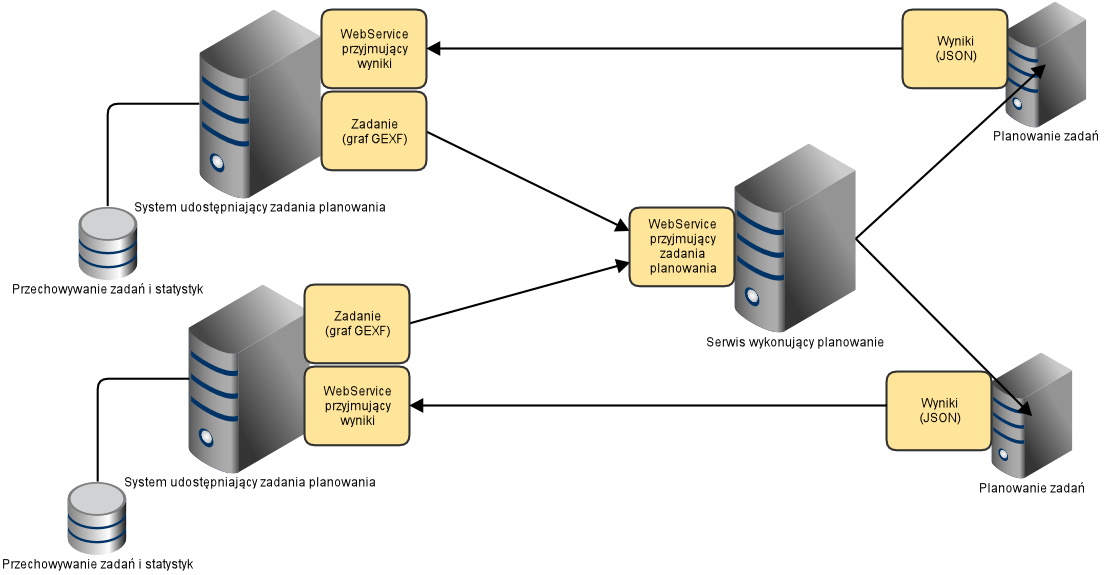
\includegraphics[width=\linewidth]{img/architektura}
	\caption{Architektura aplikacji.}
	\label{fig:architektura}
\end{figure}

\section{Web serwisy}
\label{sec:webservices}
\subsection{Web serwis przyjmujący zadania}

\subsection{Web serwis przyjmujący wyniki}

\section{Format danych}
\label{sec:data}

\subsection{GEXF}

\subsection{JSON}

\section{Algorytmy}

\subsection{BFS}
\paragraph{}
Przeszukiwanie wszerz (Breadth-first search) to jeden z najprostszych algorytmów przeszukiwania grafu. 
Przechodzenie grafu rozpoczyna się od zadanego wierzchołka i polega na odwiedzeniu wszystkich osiągalnych z niego wierzchołków. 
Wynikiem działania algorytmu jest także drzewo przeszukiwania wszerz o korzeniu w zadanym wierzchołku, zawierające wszystkie wierzchołki do których
prowadzi droga z wierzchołka początkowego. 
Algorytm działa prawidłowo zarówno dla grafów skierowanych jak i nieskierowanych.
Nie ma jednak możliwości zastosowania go do wyznaczenia ścieżki w grafie ważonym.

\paragraph{}
Na rysunku \ref{fig:bfs} przedstawiony został wynik działania algorytmu BFS na przykładowym grafie nieważonym.

\begin{figure}[!h]
 \centering
 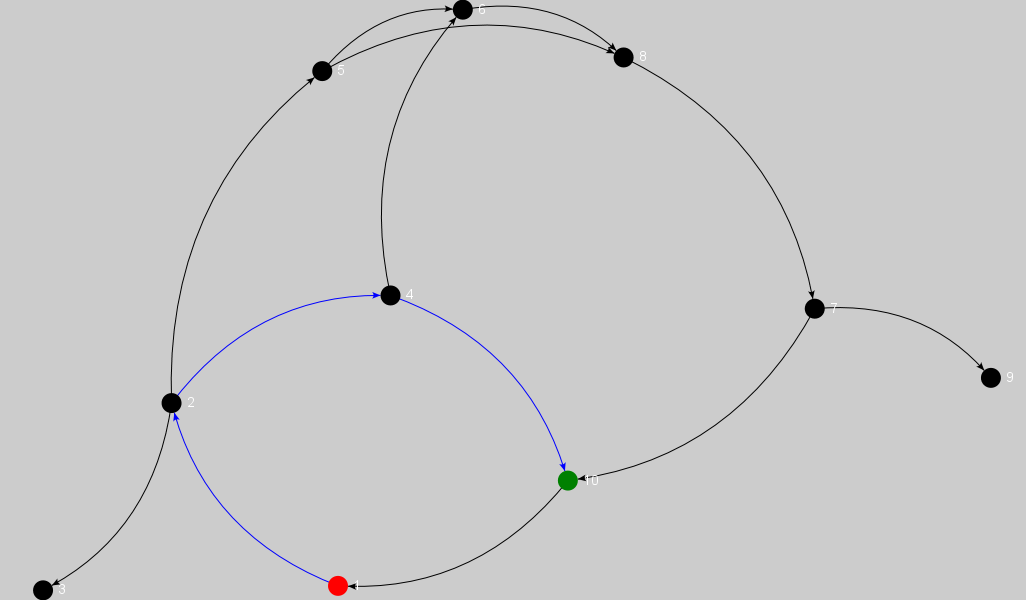
\includegraphics[width=1.0\textwidth]{algorithms/bfs}
 \caption{Wynik działania algorytmu BFS na przykładowym skierowanym, nieważonym grafie}
 \label{fig:bfs}
\end{figure}

\subsection{DFS}
\paragraph{}
Przeszukiwanie w głąb (Depth-first search) to również jeden z najprostszych algorytmów przeszukiwania grafu. 
Polega on na badaniu wszystkich krawędzi wychodzących z podanego wierzchołka w taki sposób, aby najpierw wybrać jeden z bezpośrednio przyległych
wierzchołków i zagłębić się w nim.
Po zbadaniu wszystkich krawędzi wychodzących z danego wierzchołka algorytm powraca do wierzchołka, z którego dany wierzchołek został odwiedzony.
\paragraph{}
Algorytm ten działa prawidłowo jedynie dla grafów nieskierowanych i nieważonych.

\paragraph{}
Rysunek \ref{fig:dfs} przedstawia wynik działania algorytmu przeszukiwania w głąb na nieskierowanym, nieważonym grafie.

\begin{figure}[!h]
 \centering
 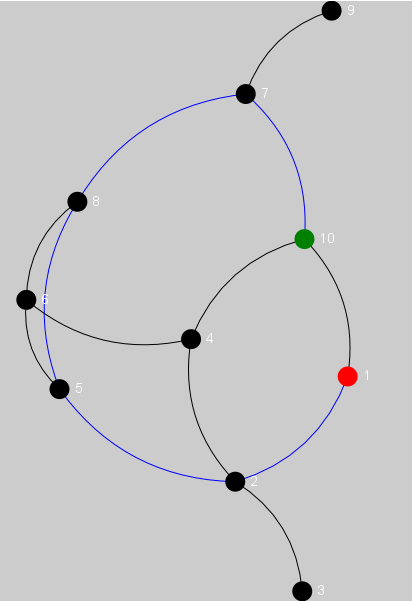
\includegraphics{algorithms/dfs}
 \caption{Wynik działania algorytmu DFS na przykładowym nieskierowanym, nieważonym grafie}
 \label{fig:dfs}
\end{figure}

\subsection{A*}
\paragraph{}
Algorytm A* to heurystyczny algorytm znajdowania najkrótszej ścieżki w grafie ważonym z dowolnego wierzchołka do wierzchołka spełniającego określony
warunek zwany testem celu. 
Algorytm jest zupełny i optymalny, w tym sensie, że znajduje ścieżkę, jeśli tylko taka istnieje, i przy tym jest to ścieżka najkrótsza. 
Stosowany głównie w dziedzinie sztucznej inteligencji do rozwiązywania problemów i w grach komputerowych do imitowania inteligentnego zachowania.
Algorytm został opisany pierwotnie w 1968 roku przez Petera Harta, Nilsa Nilssona oraz Bertrama Raphaela. 
W ich pracy naukowej został nazwany algorytmem A. 
Ponieważ jego użycie daje optymalne zachowanie dla danej heurystyki, nazwano go A*.

\paragraph{}
Na rysunku \ref{fig:aStar} przedstawiony został wynik działania algorytmu A* na przykładowym grafie.

\begin{figure}[!h]
 \centering
 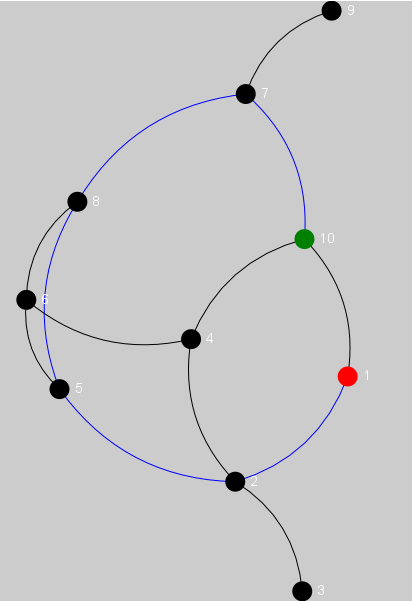
\includegraphics{algorithms/dfs}
 \caption{Wynik działania algorytmu A* na przykładowym skierowanym, ważonym grafie}
 \label{fig:aStar}
\end{figure}

\subsection{Bellman-Ford}
\paragraph{}
Algorytm Bellmana-Forda pozwala znaleźć ścieżkę o najmniejszej wadze pomiędzy zadanym wierzchołkiem początkowym a wszystkimi pozostałymi
wierzchołkami w grafie ważonym.
Idea algorytmu opiera się na metodzie relaksacji (następuje relaksacja V-1 razy każdej z krawędzi).
Algorytm ten pozwala znaleźć najkrótsze ścieżki również w grafie ważonym z ujemnymi wagami. 
Nie może jednak występować cykl o łącznej ujemnej wadze osiągalny ze źródła. 
Za tę ogólność płaci się jednak wyższą złożonością czasową. 
Działa on w czasie O(V*E).
Na algorytmie Bellmana-Forda bazuje protokół RIP - Routing Information Protocol.

\paragraph{}
Jak widać na rysunku \ref{fig:bellmanFord}, algorytm Bellmana-Forda wyznaczył poprawną ścieżkę w zadanym grafie.

\begin{figure}[!h]
 \centering
 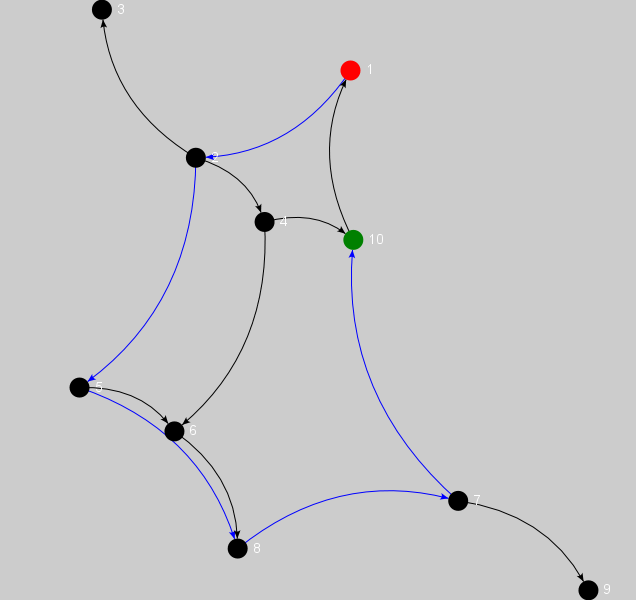
\includegraphics{algorithms/bellmanFord}
 \caption{Wynik działania algorytmu Bellmana-Forda na przykładowym skierowanym, ważonym grafie}
 \label{fig:bellmanFord}
\end{figure}

\subsection{Dijkstra}
\paragraph{}
Algorytm Dijkstry opracowany został przez holenderskiego informatyka Edsgera Dijkstrę.
Służy on do znajdowania najkrótszej ścieżki z pojedynczego źródła w grafie o nieujemnych wagach krawędzi.
Mając dany graf z wyróżnionym wierzchołkiem (źródłem) algorytm znajduje odległości od źródła do wszystkich pozostałych wierzchołków. 
Łatwo zmodyfikować go tak, aby szukał wyłącznie (najkrótszej) ścieżki do jednego ustalonego wierzchołka, po prostu przerywając działanie w momencie
dojścia do wierzchołka docelowego, bądź transponując tablicę incydencji grafu.
Algorytm Dijkstry znajduje w grafie wszystkie najkrótsze ścieżki pomiędzy wybranym wierzchołkiem a wszystkimi pozostałymi, przy okazji wyliczając
również koszt przejścia każdej z tych ścieżek.
Algorytm Dijkstry jest przykładem algorytmu zachłannego.


\paragraph{}
Jak widać na rysunku \ref{fig:dijkstra}, algorytm Dijkstry wyznaczył poprawną ścieżkę w zadanym grafie.

\begin{figure}[!h]
 \centering
 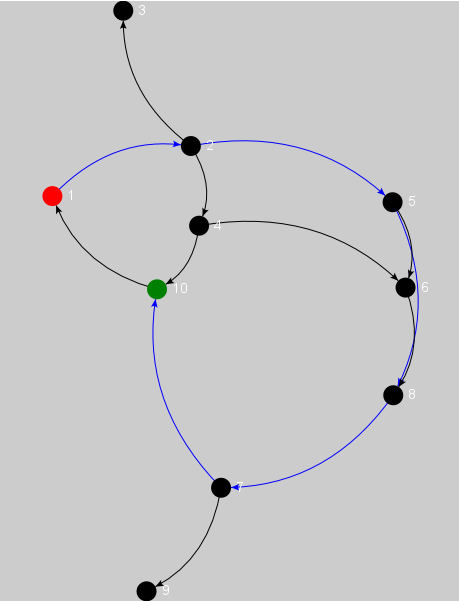
\includegraphics{algorithms/dijkstra}
 \caption{Wynik działania algorytmu Dijkstry na przykładowym skierowanym, ważonym grafie}
 \label{fig:dijkstra}
\end{figure}

\subsection{Uniform Cost}
\paragraph{}
Algorytm Uniform-cost wykorzystywany jest do przeszukiwania struktur drzewiastych oraz grafowych.
Opiera się on, na wybieraniu tego wierzchołka do odwiedzenia, który ma najmniejszą łączną sumę wag na zadanej ścieżce.

\paragraph{}
Na rysunku \ref{fig:uniformCost}, przedstawiony został wynik działania algorytmu Uniform-cost dla zadanego grafu ważonego i skierowanego.

\paragraph{}
\begin{figure}[!h]
 \centering
 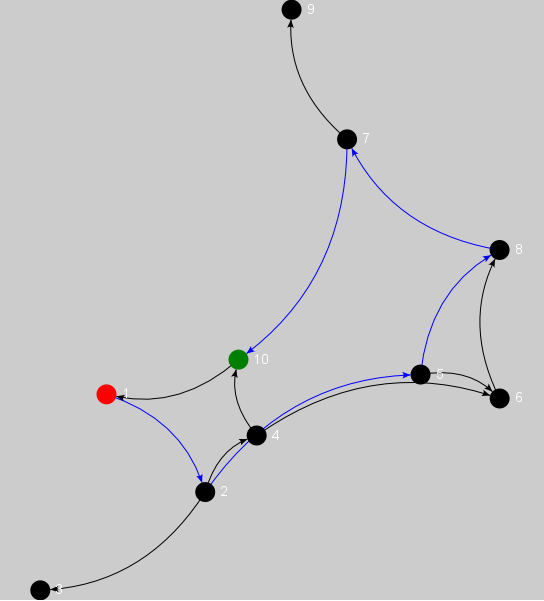
\includegraphics{algorithms/uniformCost}
 \caption{Wynik działania algorytmu Dijkstry na przykładowym skierowanym, ważonym grafie}
 \label{fig:uniformCost}
\end{figure}


\subsection{Floyd-Warshall}
\paragraph{}
Algorytm Floyda-Warshalla służy do znajdowania ścieżek z największym przepływem pomiędzy wszystkimi parami wierzchołków w grafie ważonym.
Pozwala on na szukanie ścieżek zarówno w grafach z dodatnimi jak i ujemnymi wagami krawędzi, lecz nie mogą wystąpić cykle o ujemnej wadze.
W naszej implementacji wykorzystujemy ten algorytm do wybrania ścieżki pomiędzy wierzchołkiem początkowym i końcowym bazującej na przepływie.

\paragraph{}
Jak widać na rysunku \ref{fig:floyd}, algorytm Floyda-Warshalla wyznaczył poprawną ścieżkę w zadanym grafie.
\begin{figure}[!h]
 \centering
 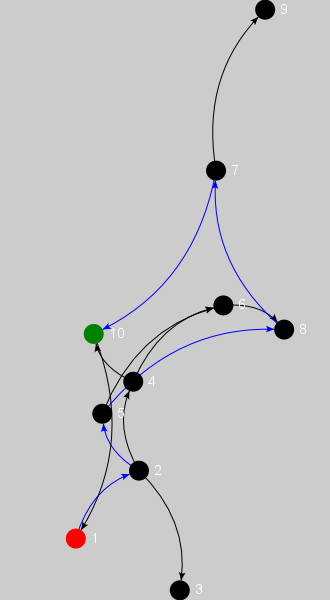
\includegraphics{algorithms/floyd}
 \caption{Wynik działania algorytmu Floyda-Warshalla na przykładowym grafie}
 \label{fig:floyd}
\end{figure}

\subsection{Prim}
\paragraph{}
Algorytm Prima oryginalnie służy do wyznaczania minimalnego drzewa rozpinającego (MST), można go jednak zaadopotować również do wyszukiwania najkrótszych ścieżek w grafie.
Wystarczy po znalezieniu minimalnego drzewa rozpinającego wyszukać w nim ścieżkę pomiędzy interesującymi nas punktami za pomocą innego, szybkiego algorytmu.
Algorytm został wynaleziony w 1930 przez czeskiego matematyka Vojtěcha Jarníka, a następnie odkryty na nowo przez informatyka Roberta C. Prima w 1957 oraz niezależnie przez Edsgera Dijkstrę w 1959. 
Z tego powodu algorytm nazywany jest również czasami algorytmem Dijkstry–Prima, algorytmem DJP, algorytmem Jarníka, albo algorytmem Prima–Jarníka.

\paragraph{}
Na rysunku \ref{fig:prim}, przedstawiono wynik działania algorytmu Prima. 
Ścieżka została poprawnie wyznaczone w zadanym nieskierowanym, ważonym grafie.
\begin{figure}[!h]
 \centering
 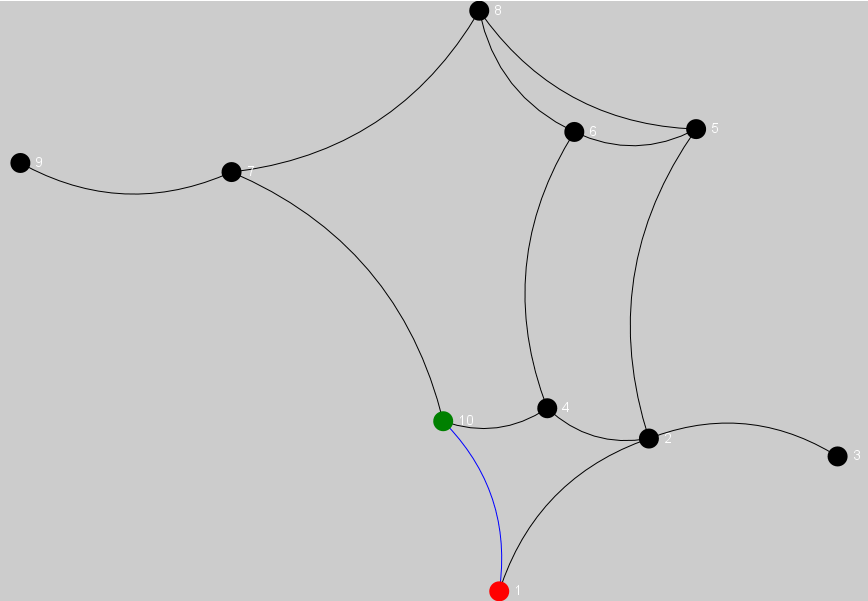
\includegraphics[width=1.0\textwidth]{algorithms/prim}
 \caption{Wynik działania algorytmu Prima na przykładowym nieskierowanym, ważonym grafie}
 \label{fig:prim}
\end{figure}

\subsection{Kruskal}
\paragraph{}
Algorytm Kruskala, podobnie jak algorytm Prima, służy do wyznaczania minimalnego drzewa rozpinającego dla grafu nieskierowanego i ważonego. 
Z wyznaczonego drzewa można następnie wyznaczyć ścieżkę pomiędzy dwoma wierzchołkami.
Innymi słowy, znajduje drzewo zawierające wszystkie wierzchołki grafu, którego waga jest najmniejsza możliwa. 
Jest to przykład algorytmu zachłannego.
Został on po raz pierwszy opublikowany przez Josepha Kruskala w 1956 roku.

\paragraph{}
Jak widać na rysunku \ref{fig:kruskal}, algorytm Kruskala wyznaczył poprawną ścieżkę w zadanym nieskierowanym, ważonym grafie.
\begin{figure}[!h]
 \centering
 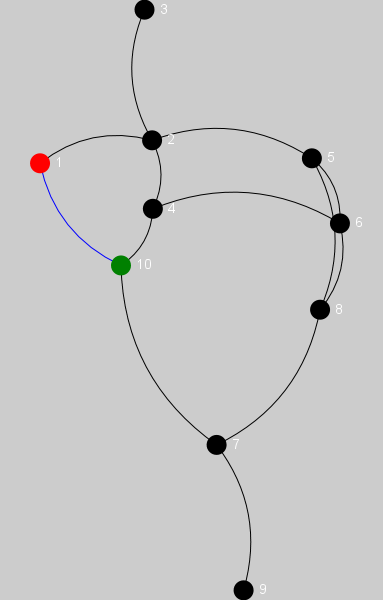
\includegraphics{algorithms/kruskal}
 \caption{Wynik działania algorytmu Kruskala na przykładowym nieskierowanym, ważonym grafie}
 \label{fig:kruskal}
\end{figure}

\section{Metryki}

\subsection{Czas wykonania}

\subsection{Zużycie pamięci}

\subsection{Waga ścieżki}

\section{Enterprise Integration Patterns}
W naszym projekcie wykorzystaliśmy cztery różne biblioteki do obliczeń grafowych. 
Każda z nich posiadała inną reprezentację danych. Wykorzystane biblioteki to:

\begin{itemize}
 \item JUNG
 \item GeoTools
 \item aima-java
 \item JGraphT
\end{itemize}

Aby umożliwić wykorzystanie algorytmów pochodzących z tych bibliotek, potrzebne było dokonanie transformacji przychodzących danych wejściowych z
formatu GEXF do formatu wykorzystywanego przez daną bibliotekę.
W tym celu skorzystaliśmy ze wzorców projektowych Enterprise Integration Patterns zaproponowanych w \cite{hohpe2004enterprise}.

\subsection{Normalizer}
Wzorzec projektowy Normalizer wykorzystuje Message Router aby skierować przychodzącą wiadomość do odpowiadającego jej Message Translatora.
Wymaga to, aby Message Router wykrył typ przesłanej wiadomości i na tej podstawie skierował ją w odopowienie miejsce.
Sytuacja została przedstawiona na rysunku \ref{fig:normalizer}

\begin{figure}[!h]
 \centering
 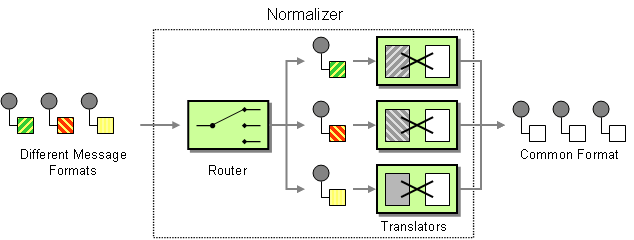
\includegraphics[width=1.0\textwidth]{eip/Normalizer}
 \caption{Wzorzec Normalizer}
 \label{fig:normalizer}
\end{figure}

\subsection{Message Router}
Worzec Message Router zapewnia przekazanie przychodzącej wiadomości do odpowiedniej kolejki w której odbędzie się dalsze przetwarzanie wiadomości.
Dokonuje się to, na podstawie wykrytego typu wiadomości.
Sytuacja została przedstawiona na rysunku \ref{fig:messageRouter}

\begin{figure}[!h]
 \centering
 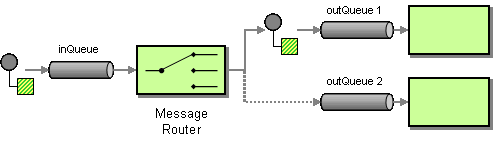
\includegraphics[width=1.0\textwidth]{eip/MessageRouter}
 \caption{Wzorzec Message Router}
 \label{fig:messageRouter}
\end{figure}

\subsection{Message Translator}
Wzorzec projektowy Message Translator wykorzystywany jest do transformacji przychodzącej wiadomości do określonego formatu wyjściowego.
Symbolicznie zostało to przedstawione na rysunku \ref{fig:messageTranslator}

\begin{figure}[!h]
 \centering
 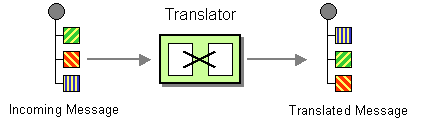
\includegraphics{eip/MessageTranslator}
 \caption{Wzorzec Message Translator}
 \label{fig:messageTranslator}
\end{figure}

\section{Uruchamianie zadań}
